%Be written in English, and submitted as a PDF document with a maximum file size of 5 MB and a guideline length of between 1500 and 3000 words (a few less or more is permissible provided all other requirements are met). You can save Microsoft Word 2016 documents in PDF format, and there are numerous online tools to convert documents to PDF.
%Start with an executive summary or overview section that concisely summarizes the analysis you performed during this project, and the conclusions you reached.
%Continue by describing the data, the process used to explore and analyze it, and the key findings, conclusions, and recommendations you reached.
%Support your conclusions by presenting statistics and visualizations.
%Be submitted by 23:59 on November 25th (UTC) to allow time for peer grading. Note that the deadline shown in the course outline reflects the final deadline for grading your fellow students' reports, not for submitting your own report. 
\documentclass[a4paper,10pt,notitlepage]{article}
\usepackage{helvet}
\usepackage{amsmath}
\usepackage{graphicx}
\usepackage{float}
\usepackage{enumitem}
\usepackage{adjustbox}
\usepackage{xcolor}

\renewcommand{\familydefault}{\sfdefault}
\usepackage[scale=.8]{geometry} % use 80% of the page
\usepackage[compact]{titlesec}

\begin{document}

\title{Analysis of Home Mortgage Rate}
\author{Yang Jiao}
\date{November, 2019}

\maketitle

\section{Executive summary}  % or overview
This report presents an analysis of data concerning
how demographics, location, property type, lender and other factors are related to the mortgage rate offered to applicants.
The analysis is based on 200,000 observations from home mortgage disclosure act (HMDA) data, each containing specific characteristics of an loan application.

Potential relationships between characteristics and rate spread were identified by statistical analysis and data visualization. 
A model to predict this rate for loan applicants was created. 

The author reached the following conclusions based on the analysis and modeling:
\begin{itemize}
\item The most affecting variables are loan information features, including property type, loan amount, lender and loan type. Specifically, 
    \subitem \textbf{Property types} Manufactured housing has higher rate spread than family housing.
    \subitem \textbf{Lenders} Some lenders have higher rate spread.
    \subitem \textbf{Loan types} FHA-insured loan has lower rate spread than conventional ones.
    \subitem \textbf{Loan amount} High loan amount is related to low rate spread. Low loan amount corresponds to wide range of rate spread.
\item An efficient prediction also rely on other loan information, applicant information, demographics and property location.
\end{itemize}

\section{Data exploration and analysis}

This data analysis starts from understanding individual feature meanings and statistics. 
Then relationships among these features and the dependence of rate spread on those features are studied.

\subsection{Individual Feature Statistics}

The targeted variable is rate spread, which is discrete numerical value. 
The rate spread distributes mainly from 1.0 to 8.0 and has outliers from 9.0 to 32.0 and then a few cases in 99.0. 
The distribution of rate spread is plotted in Fig.~\ref{fig:rate_spread}. The counts of other values are at least two dimensional smaller and can not be shown in the same plot.

\begin{figure}[htb]
\centering
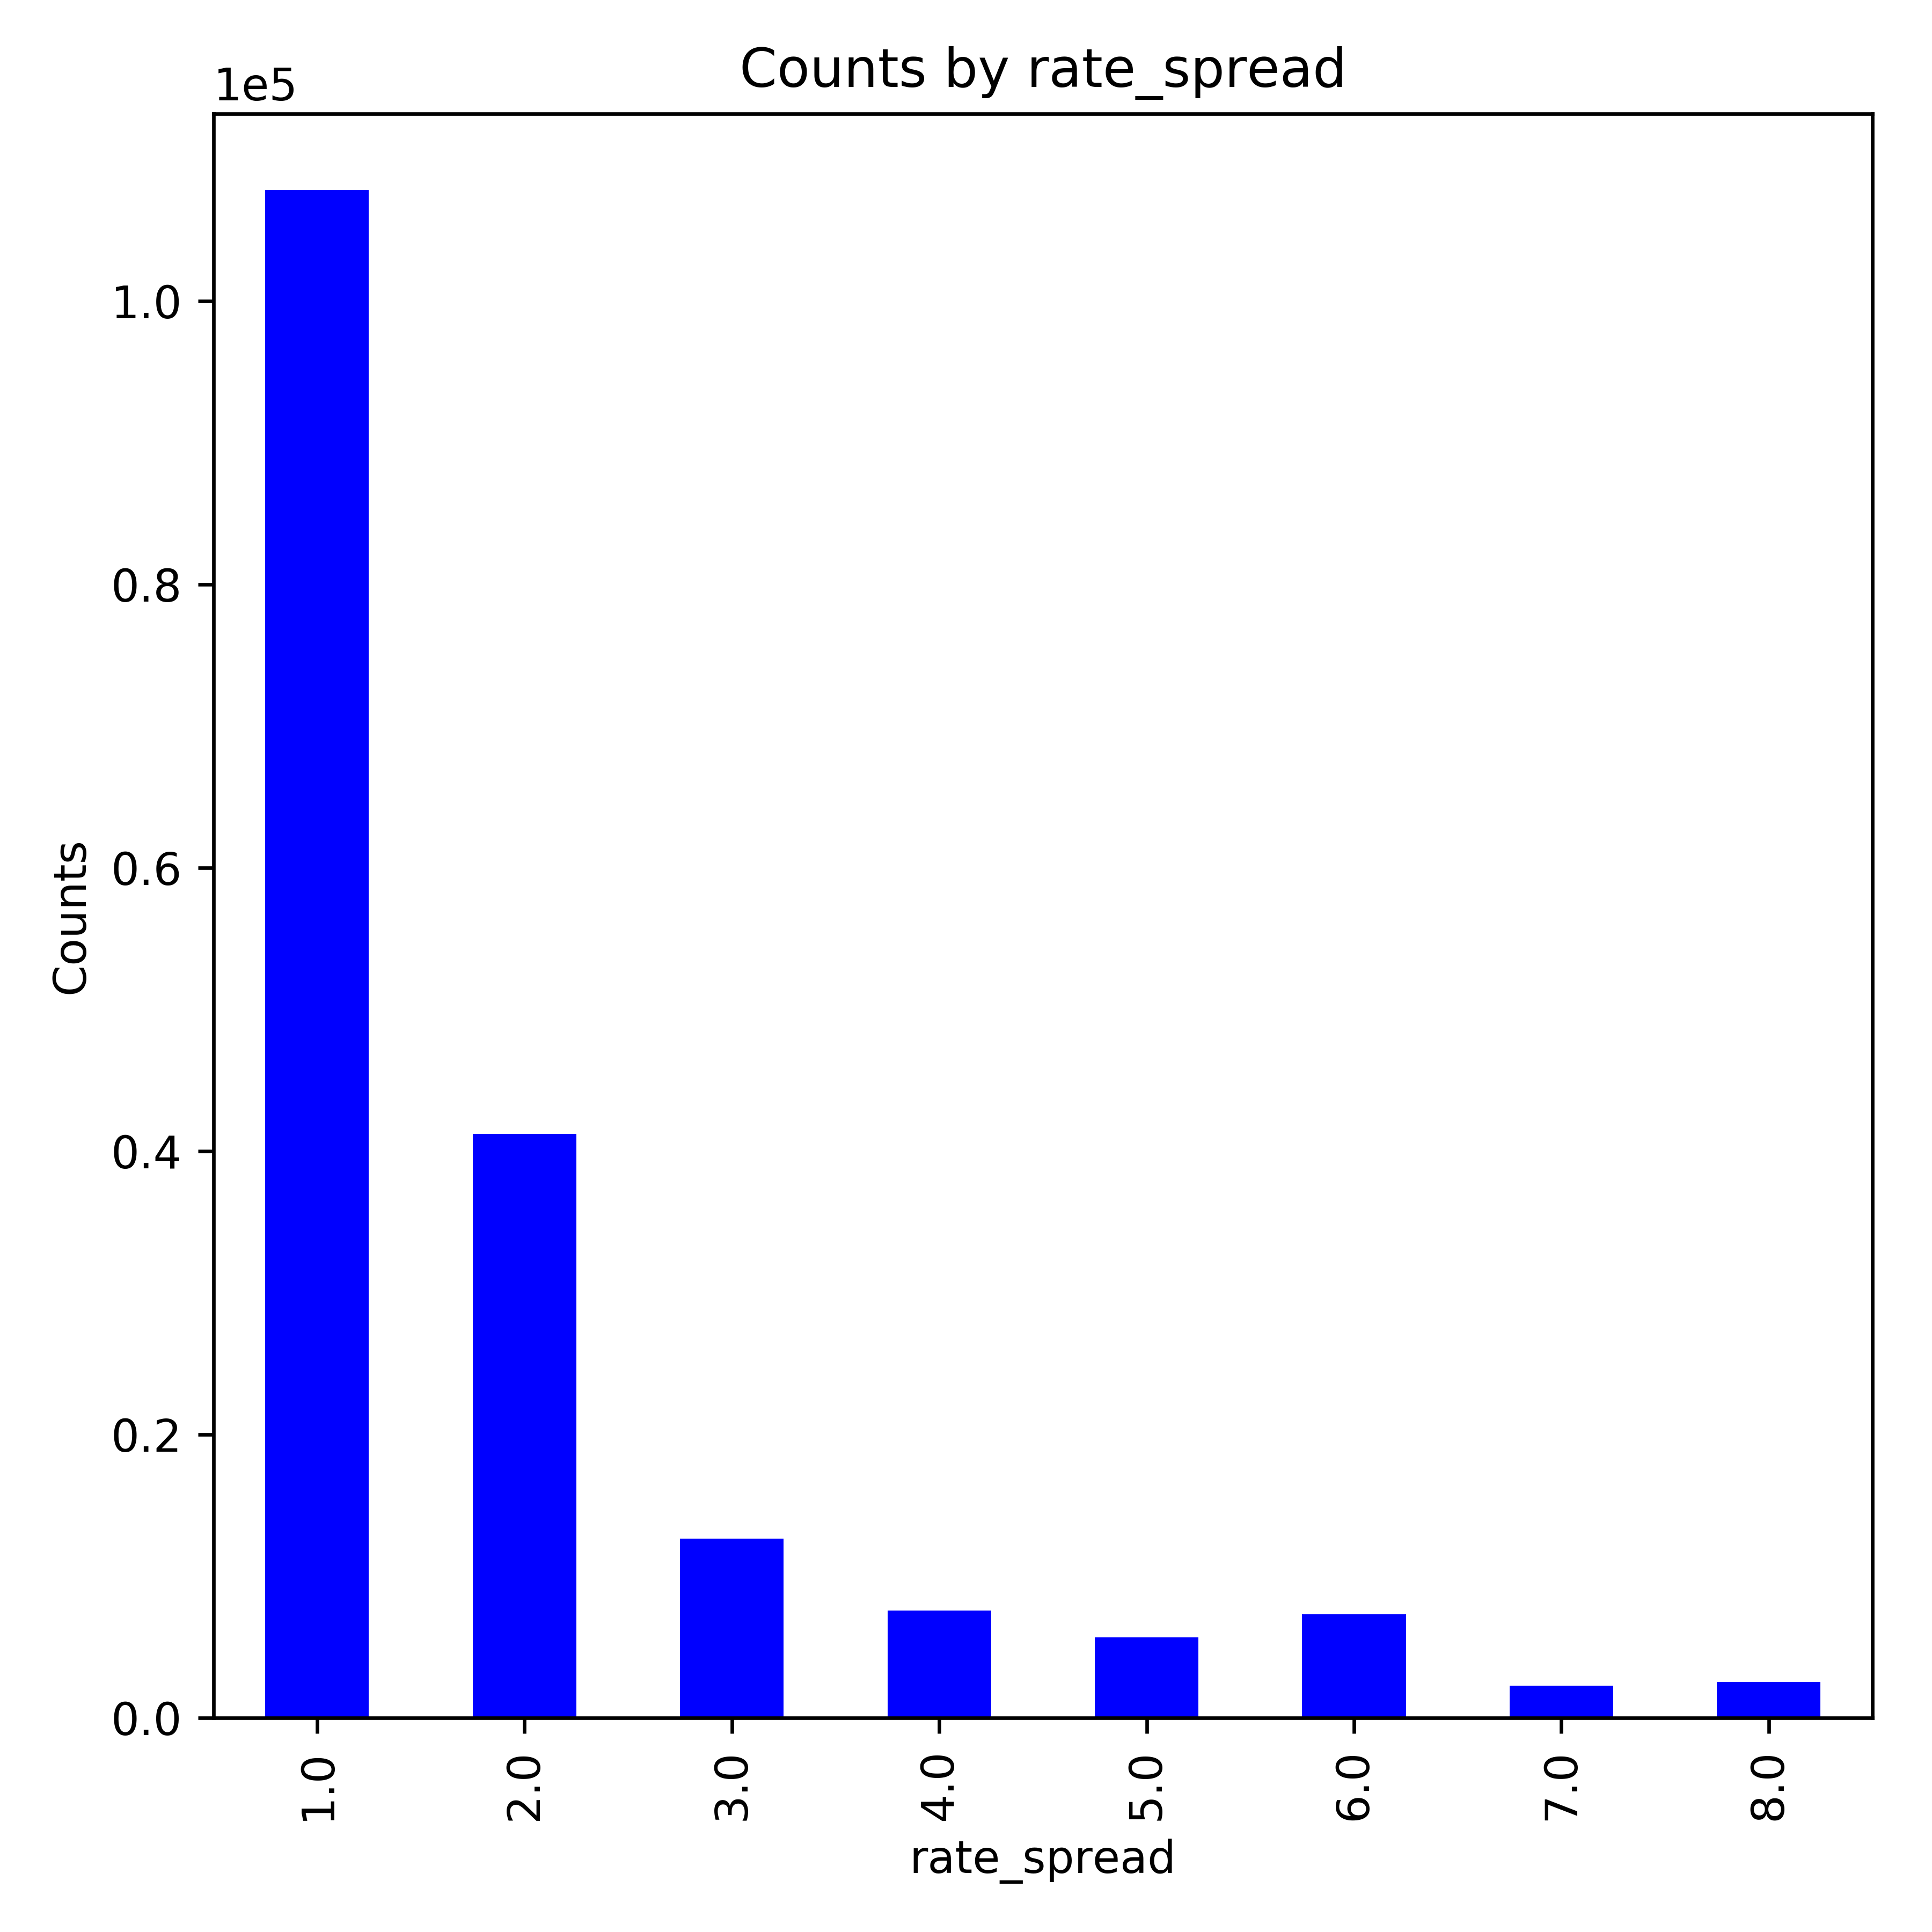
\includegraphics[width=0.6\textwidth]{rate_spread_counts.png}
\caption{The distribution of rate spread in training dataset. Values with much fewer count are not shown here.}
\label{fig:rate_spread}
\end{figure}

The dataset contains the following numerical columns:

\begin{itemize}
\item Loan information
    \subitem Loan amount (K\$)
\item Applicant information
    \subitem Gross Annual Income (K\$)
\item Census information
    \subitem Population
    \subitem Minority population ($\%$)
    \subitem FFIEC median family income (\$) for the MSA/MD
    \subitem Tract to MSA/MD median family income ($\%$) 
    \subitem Number of owner occupied units
    \subitem Number of 1- to 4-family units
\end{itemize}

Besides these numerical columns, it also has the following categorical features. Some of the counts are listed in square brackets:

\begin{itemize}
\item{ Property location, which includes}
    \subitem{ MSA/MD      }
    \subitem{ State  }
    \subitem{ County  }
\item{ Loan information  }
    \subitem{ Lender  }
    \subitem{ Loan type -- Conventional [86,929], FHA-insured [97,478], VA-guaranteed [1,030] and FSA/RHS [1,860]  }
    \subitem{ Property type -- One to four-family [158,334], manufactured housing [28,964] and multifamily [0] }
    \subitem{ Loan purpose -- Home purchase [143,145], home improvement [10,885] and refinancing [33,267] }
    \subitem{ Owner occupancy -- Owner-occupied as a principal dwelling [176,877], not owner-occupied [10,269] and not applicable [151]  }
    \subitem{ Preapproval -- Preapproval was requested [8,748], was not requested [41,006] or not applicable [137,543]  }
\item{ Applicant information  }
    \subitem{ Ethnicity  }
    \subitem{ Race  }
    \subitem{ Sex  }
    \subitem{ Co-applicant  }
\end{itemize}

Among the categorical features, the property location features, including MSA/MD, state and county have large amount of unique values, and some values only have a few entries.
It is the same case for lender feature. 
These features are included and values with few entries will be selected out in feature selection processes.
Other variables also have highly unbalanced distribution. 
In the following plots, only values with at least $1\%$ frequency are presented.

\subsection{Feature correlations}

The population, number of owner occupied units and number of 1- to 4- family units are linear related to each other as shown in Fig.~\ref{fig:cor2}.
No significant correlations are observed among other numerical features.
This observation was confirmed by the calculated correlation (Table~\ref{tab:corr}). 
The population, number of owner occupied units and number of 1- to 4-family units have correlation coefficients of each pair higher than 0.8. All the other correlation coefficients are lower than 0.5.

Loan amount and applicant income are highly right-screwed distributions as shown in Fig.~\ref{fig:cor1}. Higher loan amount is related to higher applicant income, with correlation coefficient of 0.45. 

\begin{figure}[H]
\centering
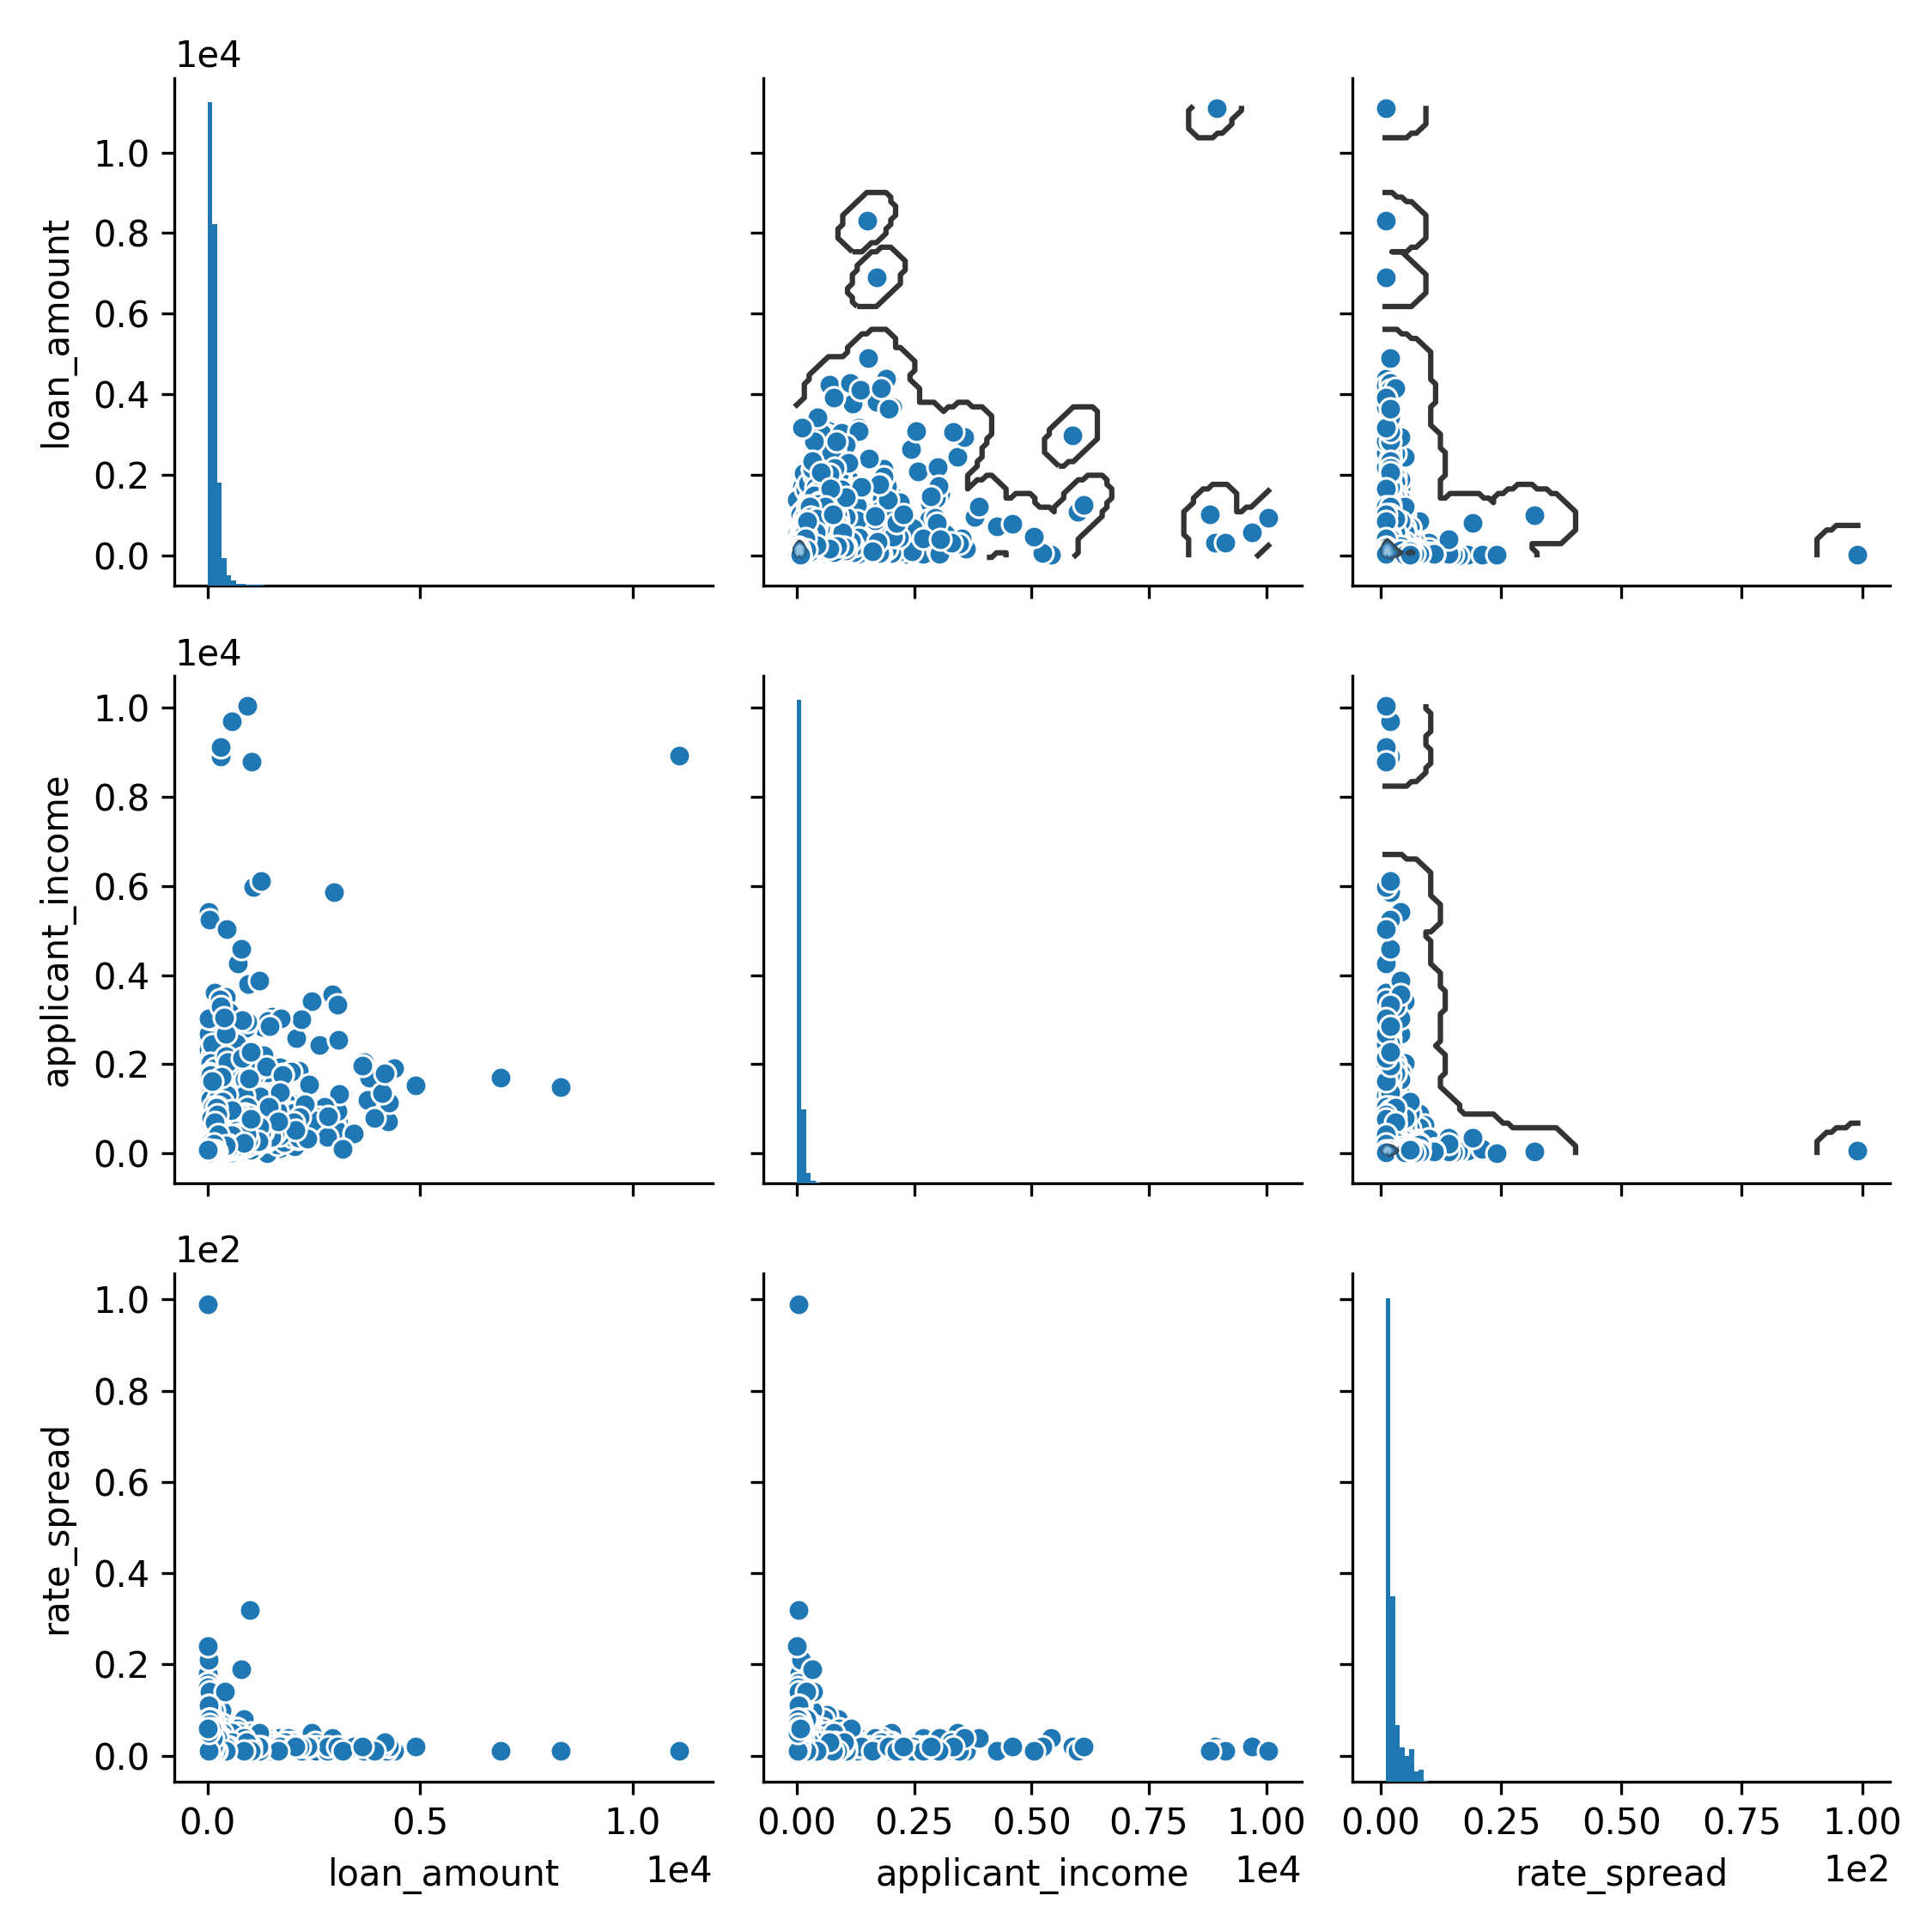
\includegraphics[width=0.6\textwidth]{hmda_pairwise_1_rate.png}
\caption{The correlation between loan amount, applicant income and rate spread.}
\label{fig:cor1}
\end{figure}

\begin{figure}[H]
\centering
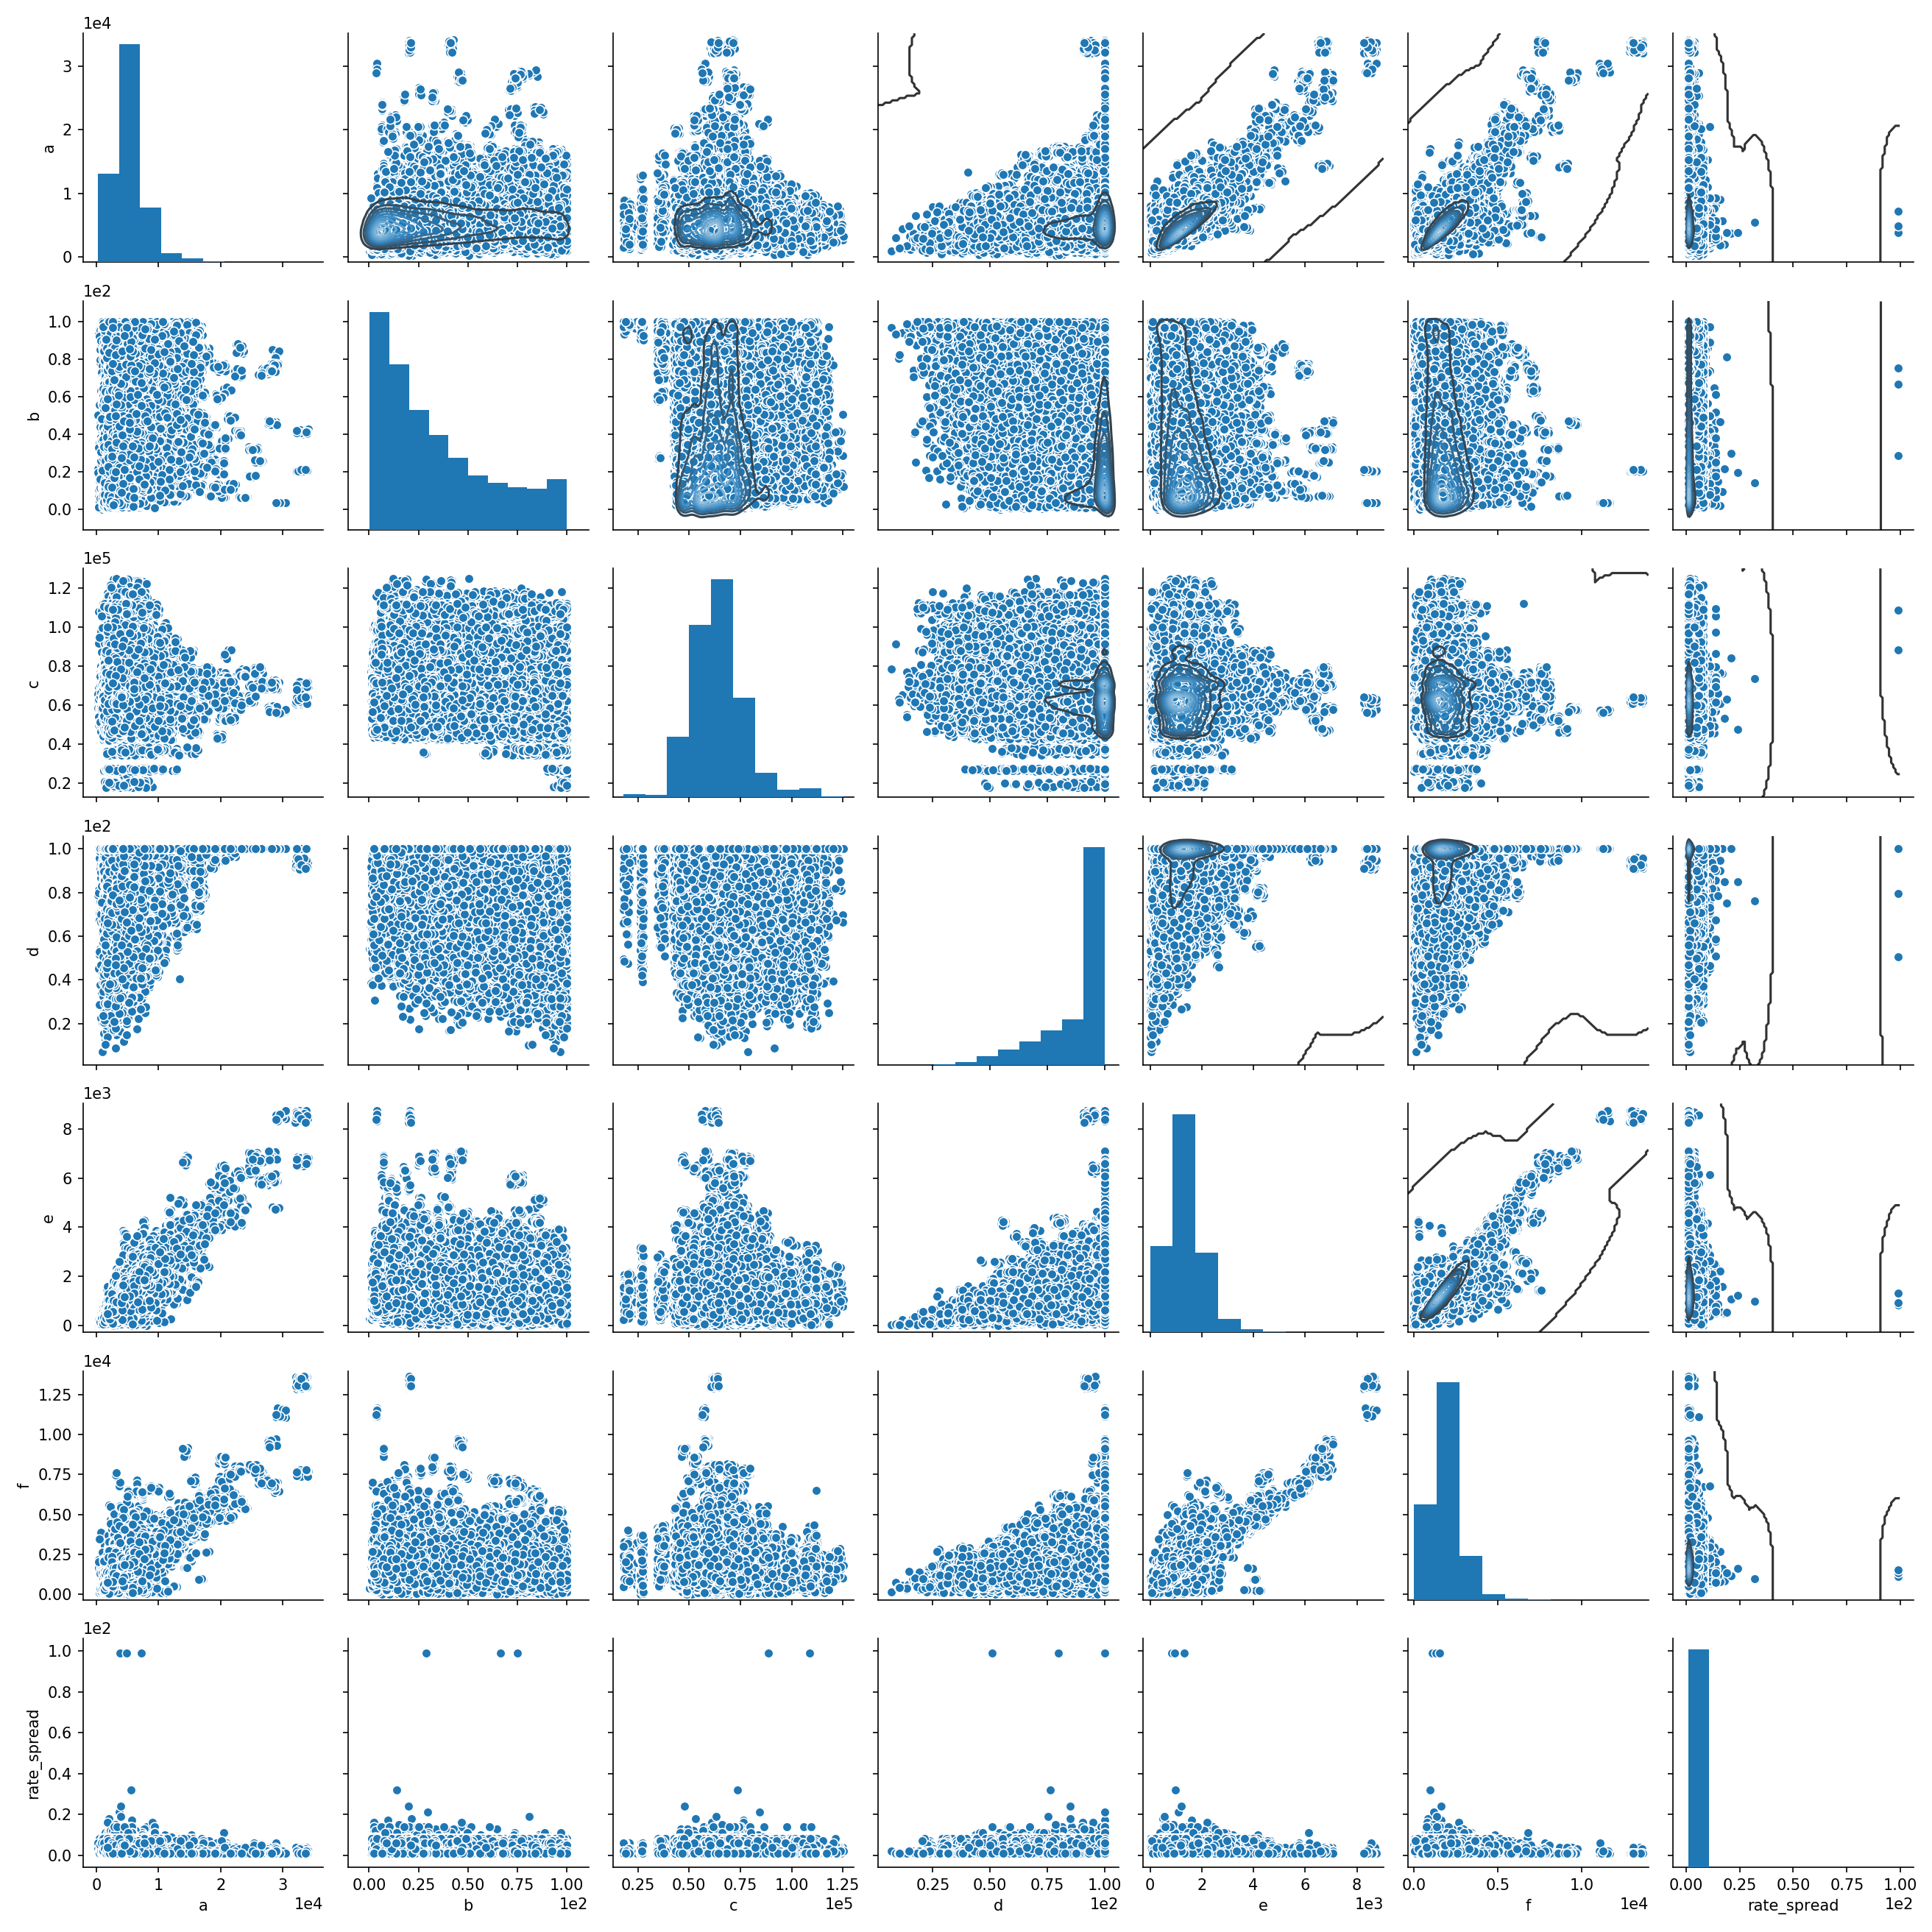
\includegraphics[width=1.0\textwidth]{hmda_pairwise_2_rate.png}
\caption{The correlation between census information variables.
a: population; b: minority\_population\_pct; c: ffiecmedian\_family\_income; 
d: tract\_to\_msa\_md\_income\_pct; e: number\_of\_owner\_occupied\_units; f: number\_of\_1\_to\_4\_family\_units.
}
\label{fig:cor2}
\end{figure}

\begin{table}
\centering
\caption{The correlation table of numerical variables.}
\label{tab:corr}
\begin{tabular}{r{1cm}r{1cm}r{1cm}r{1cm}r{1cm}r{1cm}r{1cm}r{1cm}r{1cm}r{1cm}}
% & loan\_amount  & applicant\_income  & population  & minority\_population\_pct  & ffiecmedian\_family\_income  & tract\_to\_msa\_md\_income\_pct  & number\_of\_owner\_occupied\_units  & number\_of\_1\_to\_4\_family\_units  & rate\_spread \\
\hline \hline
 & a & b & c & d & e & f & g & h & i \\
 \hline
 a  & 1.000  & \textcolor{orange}{0.450}  & 0.070  & 0.098  & 0.245  & 0.114  & 0.028  & -0.025  & -0.255 \\
 b  & \textcolor{orange}{0.450}  & 1.000  & 0.014  & -0.027  & 0.089  & 0.088  & 0.023  & 0.001  & -0.019 \\
 c  & 0.070  & 0.014  & 1.000  & 0.136  & 0.028  & 0.156  & \textcolor{red}{0.856}  & \textcolor{red}{0.837}  & -0.033 \\
 d  & 0.098  & -0.027  & 0.136  & 1.000  & 0.043  & -0.415  & -0.182  & -0.130  & -0.082 \\
 e  & 0.245  & 0.089  & 0.028  & 0.043  & 1.000  & -0.132  & 0.008  & -0.107  & -0.094 \\
 f  & 0.114  & 0.088  & 0.156  & -0.415  & -0.132  & 1.000  & 0.369  & 0.229  & 0.012 \\
 g  & 0.028  & 0.023  & \textcolor{red}{0.856}  & -0.182  & 0.008  & 0.369  & 1.000  & \textcolor{red}{0.905}  & 0.009 \\
 h  & -0.025  & 0.001  & \textcolor{red}{0.837}  & -0.130  & -0.107  & 0.229  & \textcolor{red}{0.905}  & 1.000  & 0.026 \\
 i  & -0.255  & -0.019  & -0.033  & -0.082  & -0.094  & 0.012  & 0.009  & 0.026  & 1.000 \\
 \hline
\end{tabular}
\begin{footnotesize}
\begin{itemize}
    \item[a] loan\_amount
    \item[b] applicant\_income
    \item[c] population
    \item[d] minority\_population\_pct
    \item[e] ffiecmedian\_family\_income
    \item[f] tract\_to\_msa\_md\_income\_pct
    \item[g] number\_of\_owner\_occupied\_units
    \item[h] number\_of\_1\_to\_4\_family\_units
    \item[i] rate\_spread
\end{itemize}
\end{footnotesize}
\end{table}

\subsection{Feature dependency}

No obvious simple relationship is observed between rate spread and other variables (Fig.~\ref{fig:cor1}, Fig.~\ref{fig:cor2}).
The dependency of rate spread on some of the categorical features are plotted in Fig.~\ref{fig:rate_propertytype} -- Fig.~\ref{fig:rate_loantype}. For the property type, multifamily type does not appear in this training set. In prediction for new entries, one to four-family type and multifamily type will be accumulated together (other than manufactured housing). The new categories in property type variables will be family and manufactured housing. 




\begin{figure}[H]
\centering
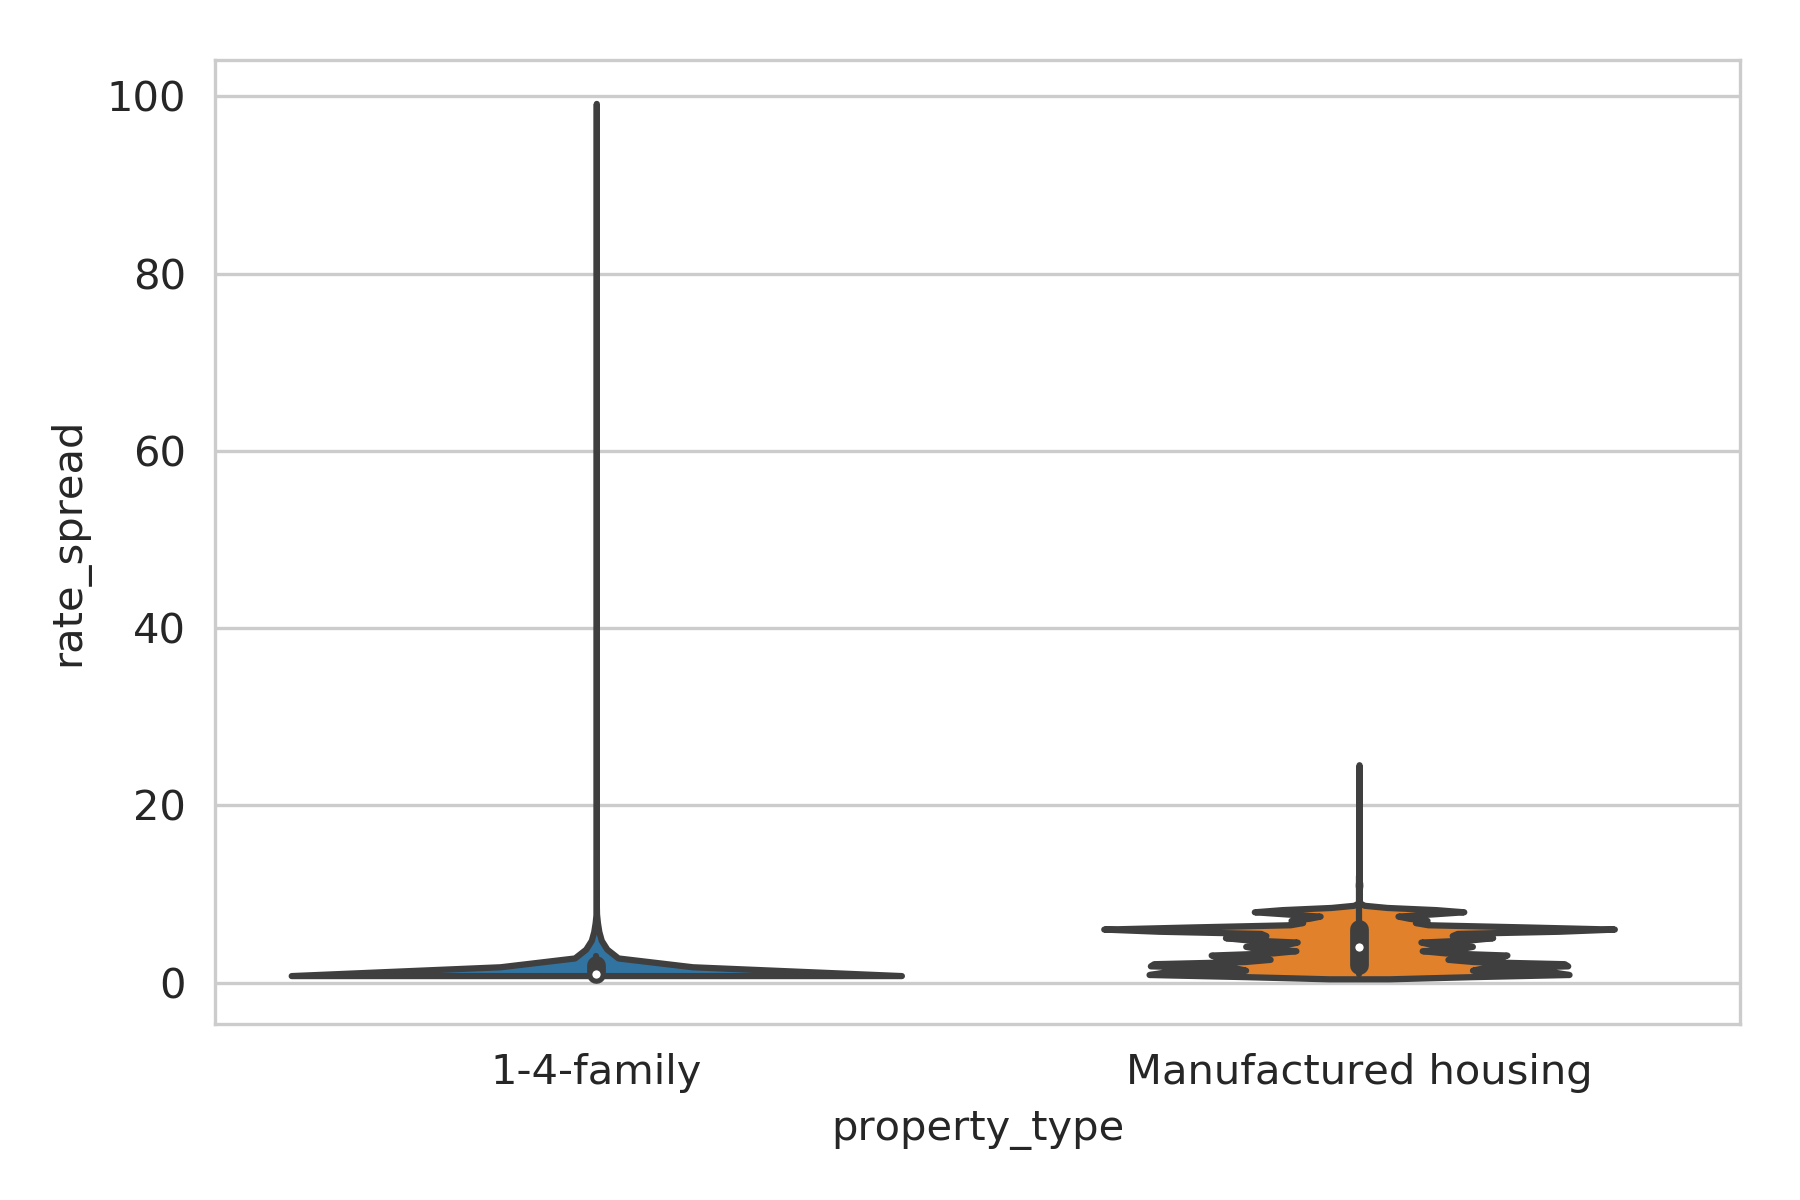
\includegraphics[width=0.6\textwidth]{hmda_violin_property_type.png}
\caption{The dependency of rate spread on property type.}
\label{fig:rate_propertytype}
\end{figure}


\begin{figure}[H]
\centering
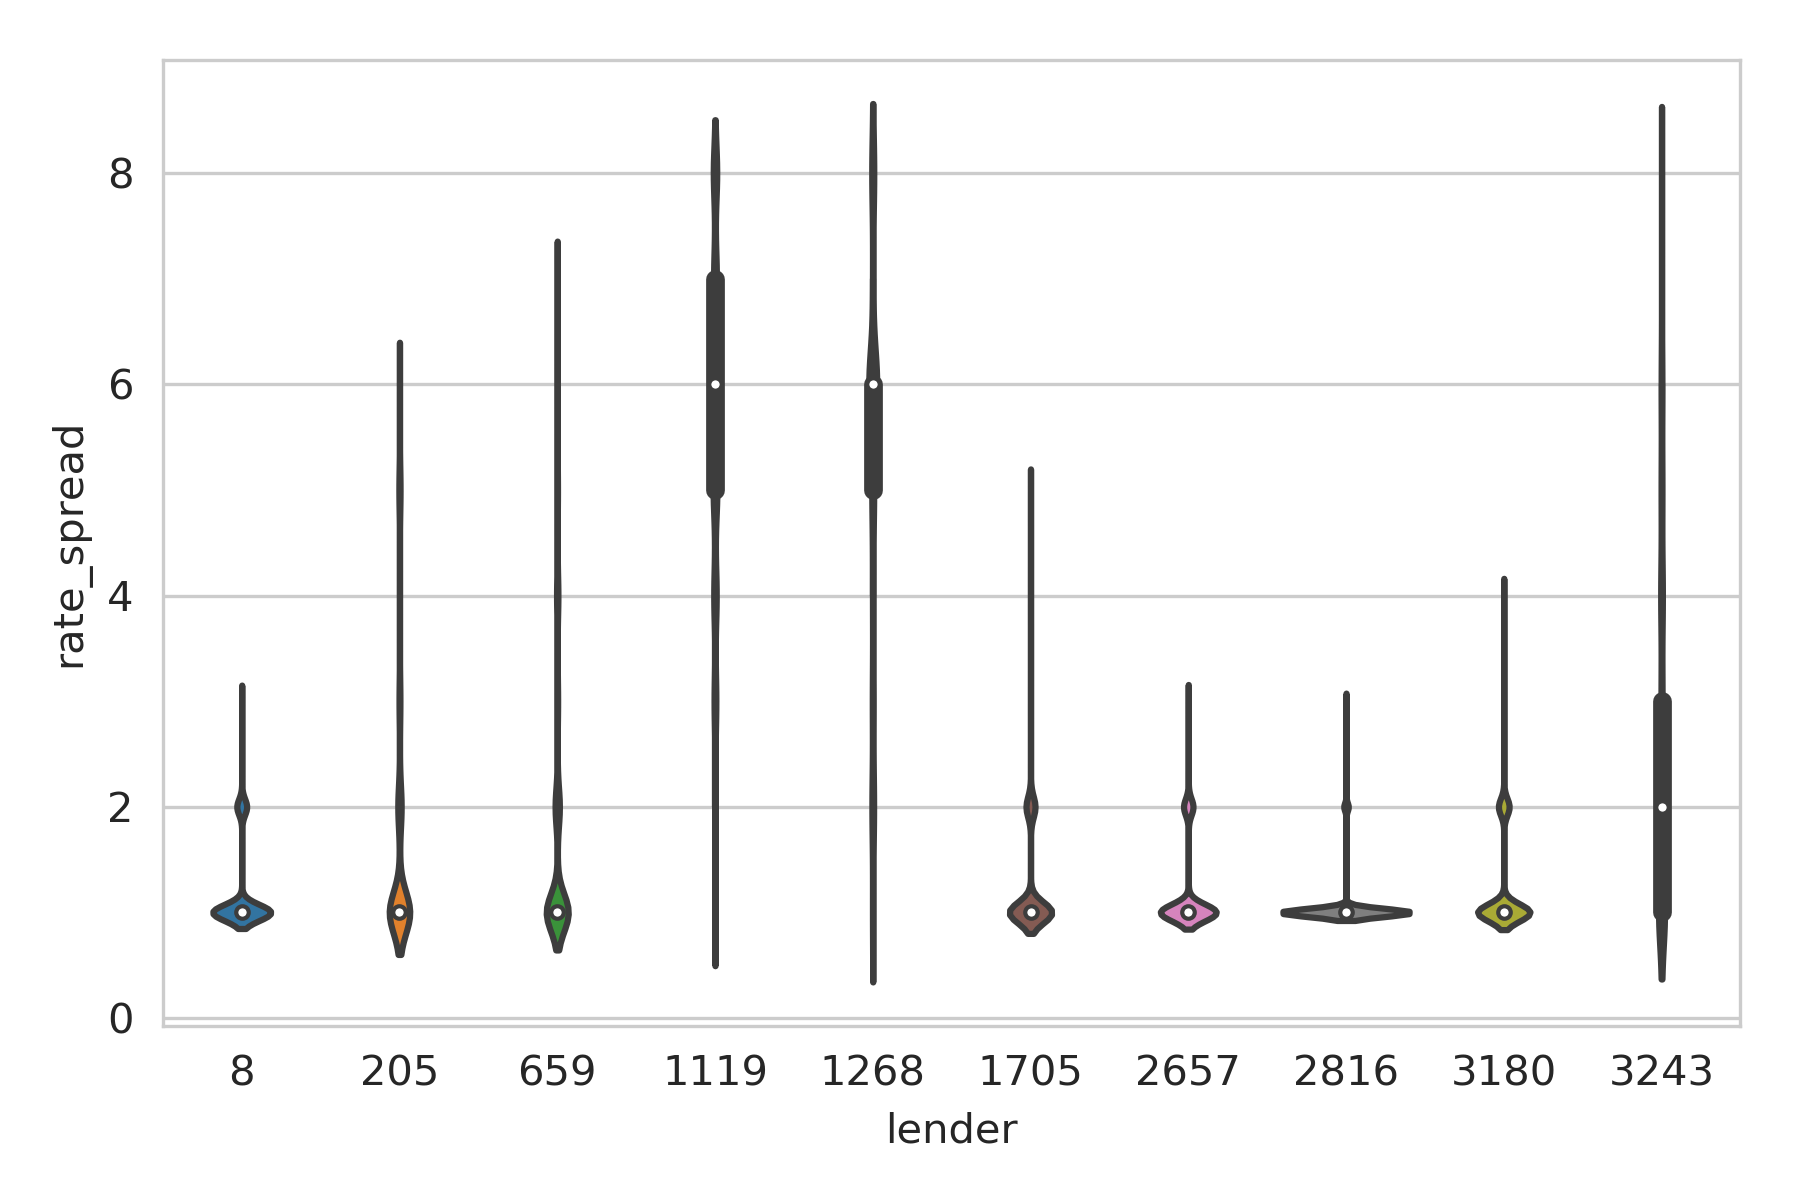
\includegraphics[width=0.6\textwidth]{hmda_violin_lender.png}
\caption{The dependency of rate spread on lender.}
\label{fig:rate_lender}
\end{figure}

\begin{figure}[H]
\centering
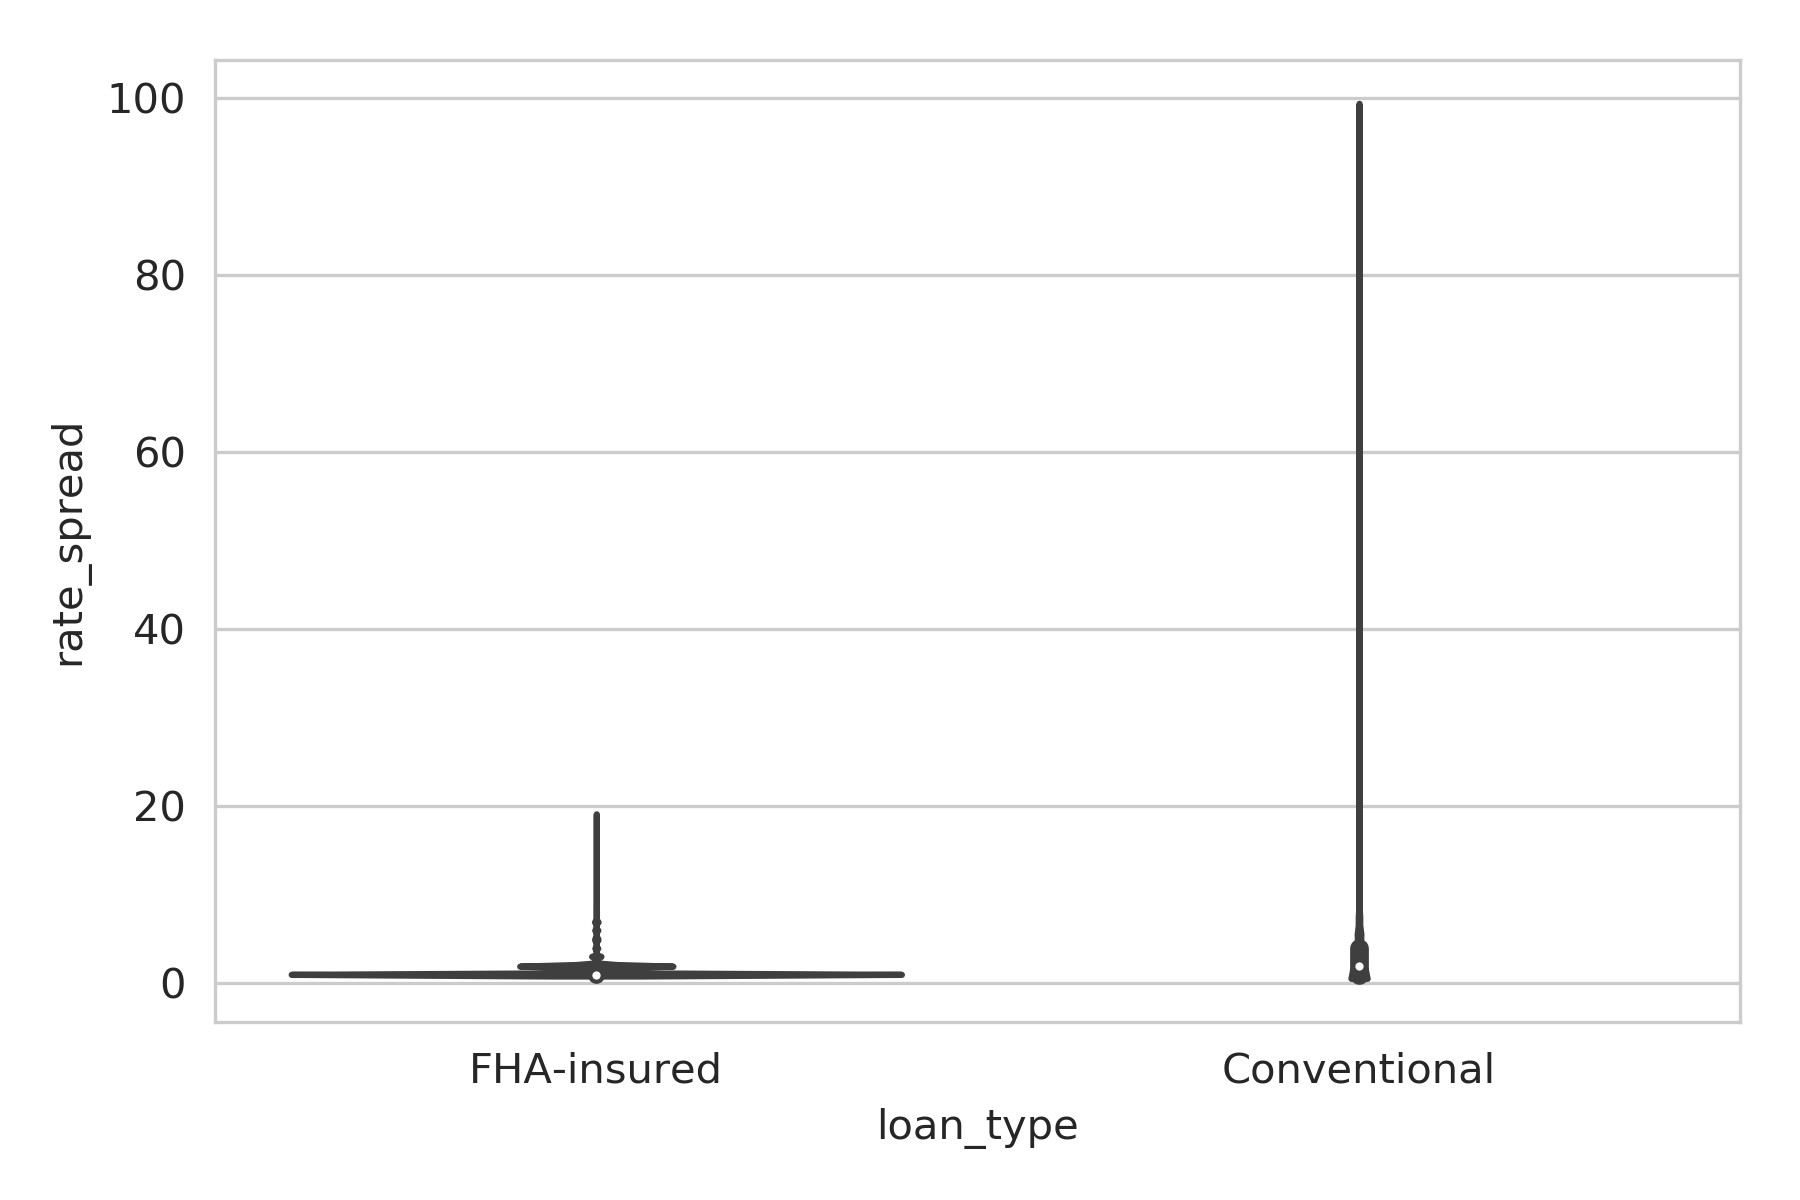
\includegraphics[width=0.6\textwidth]{hmda_violin_loan_type.png}
\caption{The dependency of rate spread on loan type.}
\label{fig:rate_loantype}
\end{figure}


\section{Key findings}

Based on the analysis of the home mortgage data, a predictive model to estimate the rate spread was created.
This dataset has large amount of features. A random forest regressor model, which usually performs good with noise and outliers, was deployed to predict the rate spread. Hyperparameters were optimized using nested cross validation method.

There are 200,000 observations in this dataset in total, among which no duplicate cases was found. 12,703 observations have missing values, which were removed from the training set. 

Categorical features were encoded into binary dummy variables using label encoding and one hot encoding. Since many categories in property location variables (MSA/MD, state, county) and lender variable have few entries, we got large number of low variance features. 
Low variance features were removed with a variance threshold of $99\%$. All of the categorical features were transformed into 122 binary dummy variables.

Numerical variables were standardized. The total number of features are 130.  

A nested cross validation with 10 subset give

\begin{itemize}
    \item Mean $R^2$: 0.659
    \item Standard deviation of $R^2$: 0.039
    \item Best estimator of random forest regressor model: 
        \subitem max\_features: 60
        \subitem min\_samples\_leaf: 10
\end{itemize}

The model was then trained with 167,297 observations and tested with the remaining 20,000 observations. A scatter plot shows the predicted rate spread and the actual rate spread (Fig.~\ref{fig:label_predicted}).
The metrics of this prediction are listed in Table~\ref{tab:metrics}.

\begin{figure}[H]
\centering
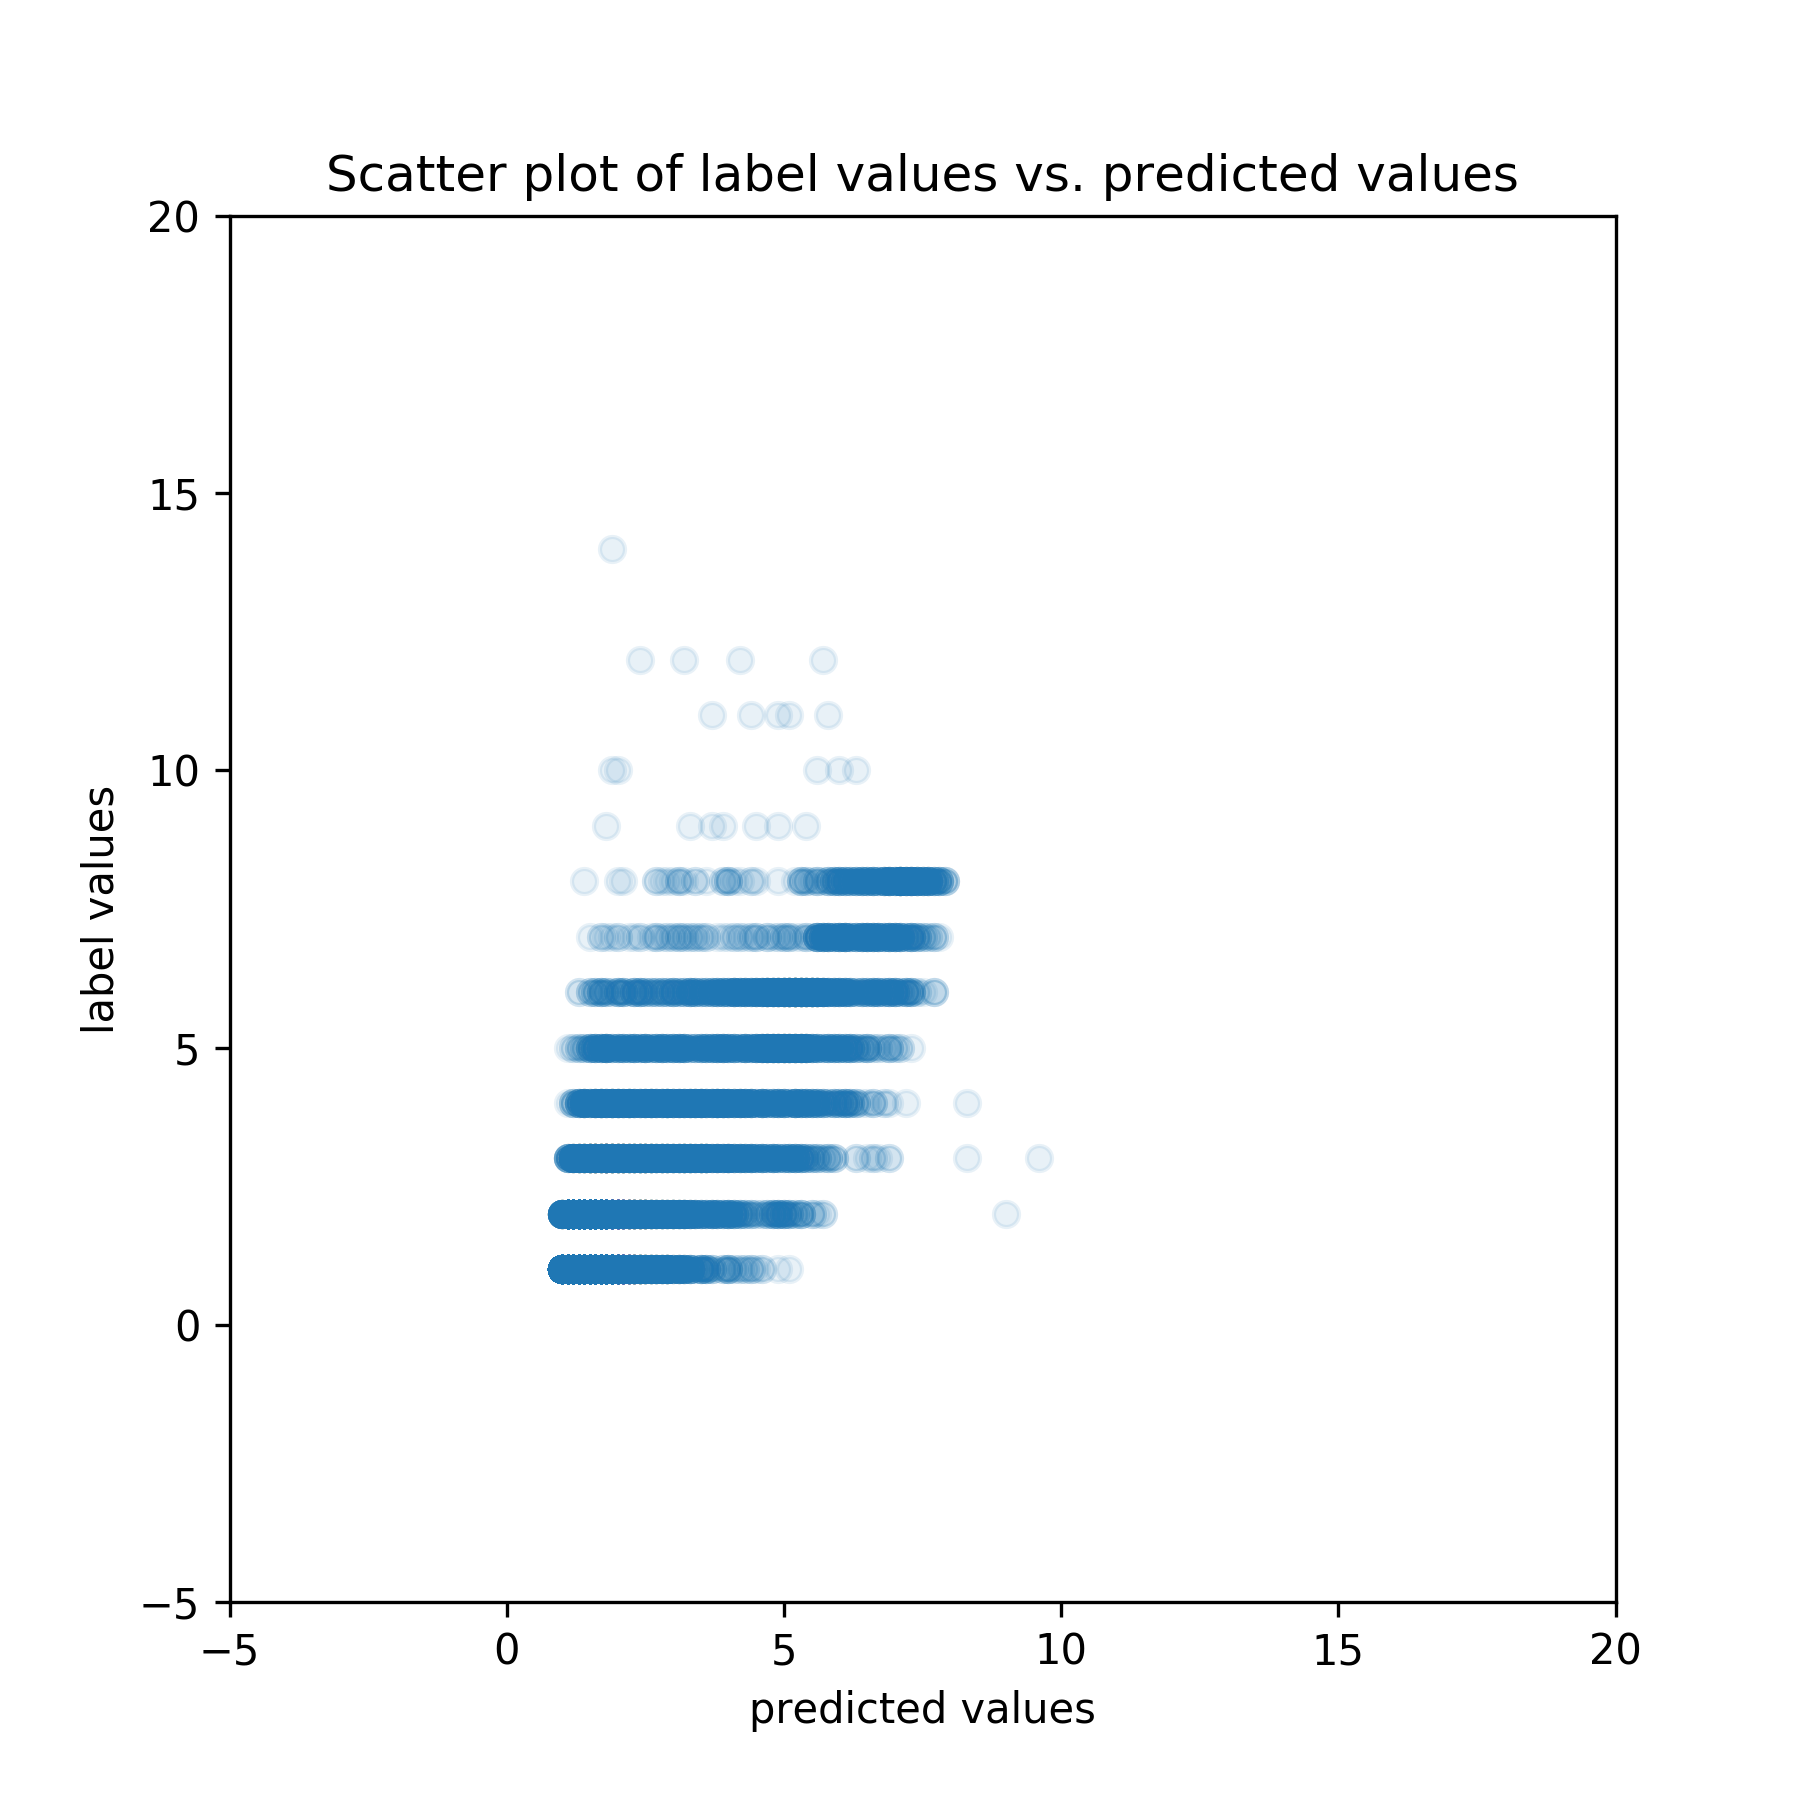
\includegraphics[width=0.6\textwidth]{label_predicted.png}
\caption{The labels versus predicted values in test set.}
\label{fig:label_predicted}
\end{figure}

\begin{table}
\centering
\caption{The metrics for the test subset using the optimized hyperparameters.}
\label{tab:metrics}
\begin{tabular}{lr}
\hline \hline
 MSE     &   1.227   \\
 RMSE    &   1.108   \\
 MAE     &   0.614    \\
 $R^2$   &   0.602    \\
\hline
\end{tabular} 
\end{table}

From Fig.~\ref{fig:res_predicted}, 
the residues do not have significant dependence on predicted values.  
A quantile quantile normal plot (Fig.~\ref{fig:qq}) follows normal distribution in general. 
It indicates that this prediction is reliable.


\begin{figure}[H]
\centering
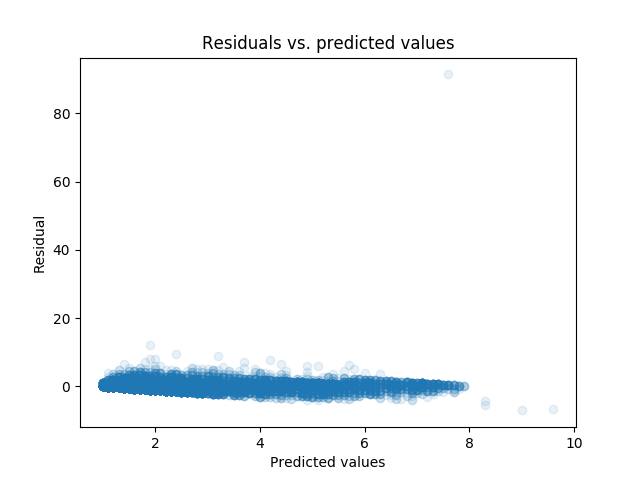
\includegraphics[width=0.6\textwidth]{res_predictedvalues.png}
\caption{The residues vs. predicted values. }
\label{fig:res_predicted}
\end{figure}

\begin{figure}[H]
\centering
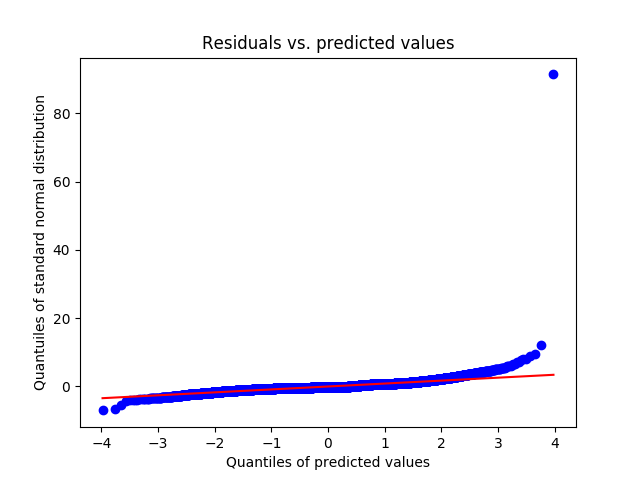
\includegraphics[width=0.6\textwidth]{quantile_quantile_normal_plot.png}
\caption{The quantile quantile normal plot for the test set.}
\label{fig:qq}
\end{figure}

The importance of the features were calculated during the random forest regressor modeling.
The importance of the leading features are plotted in Fig.~\ref{fig:importance}. This figure confirmed our analysis in previous section.  

\begin{figure}[H]
\centering
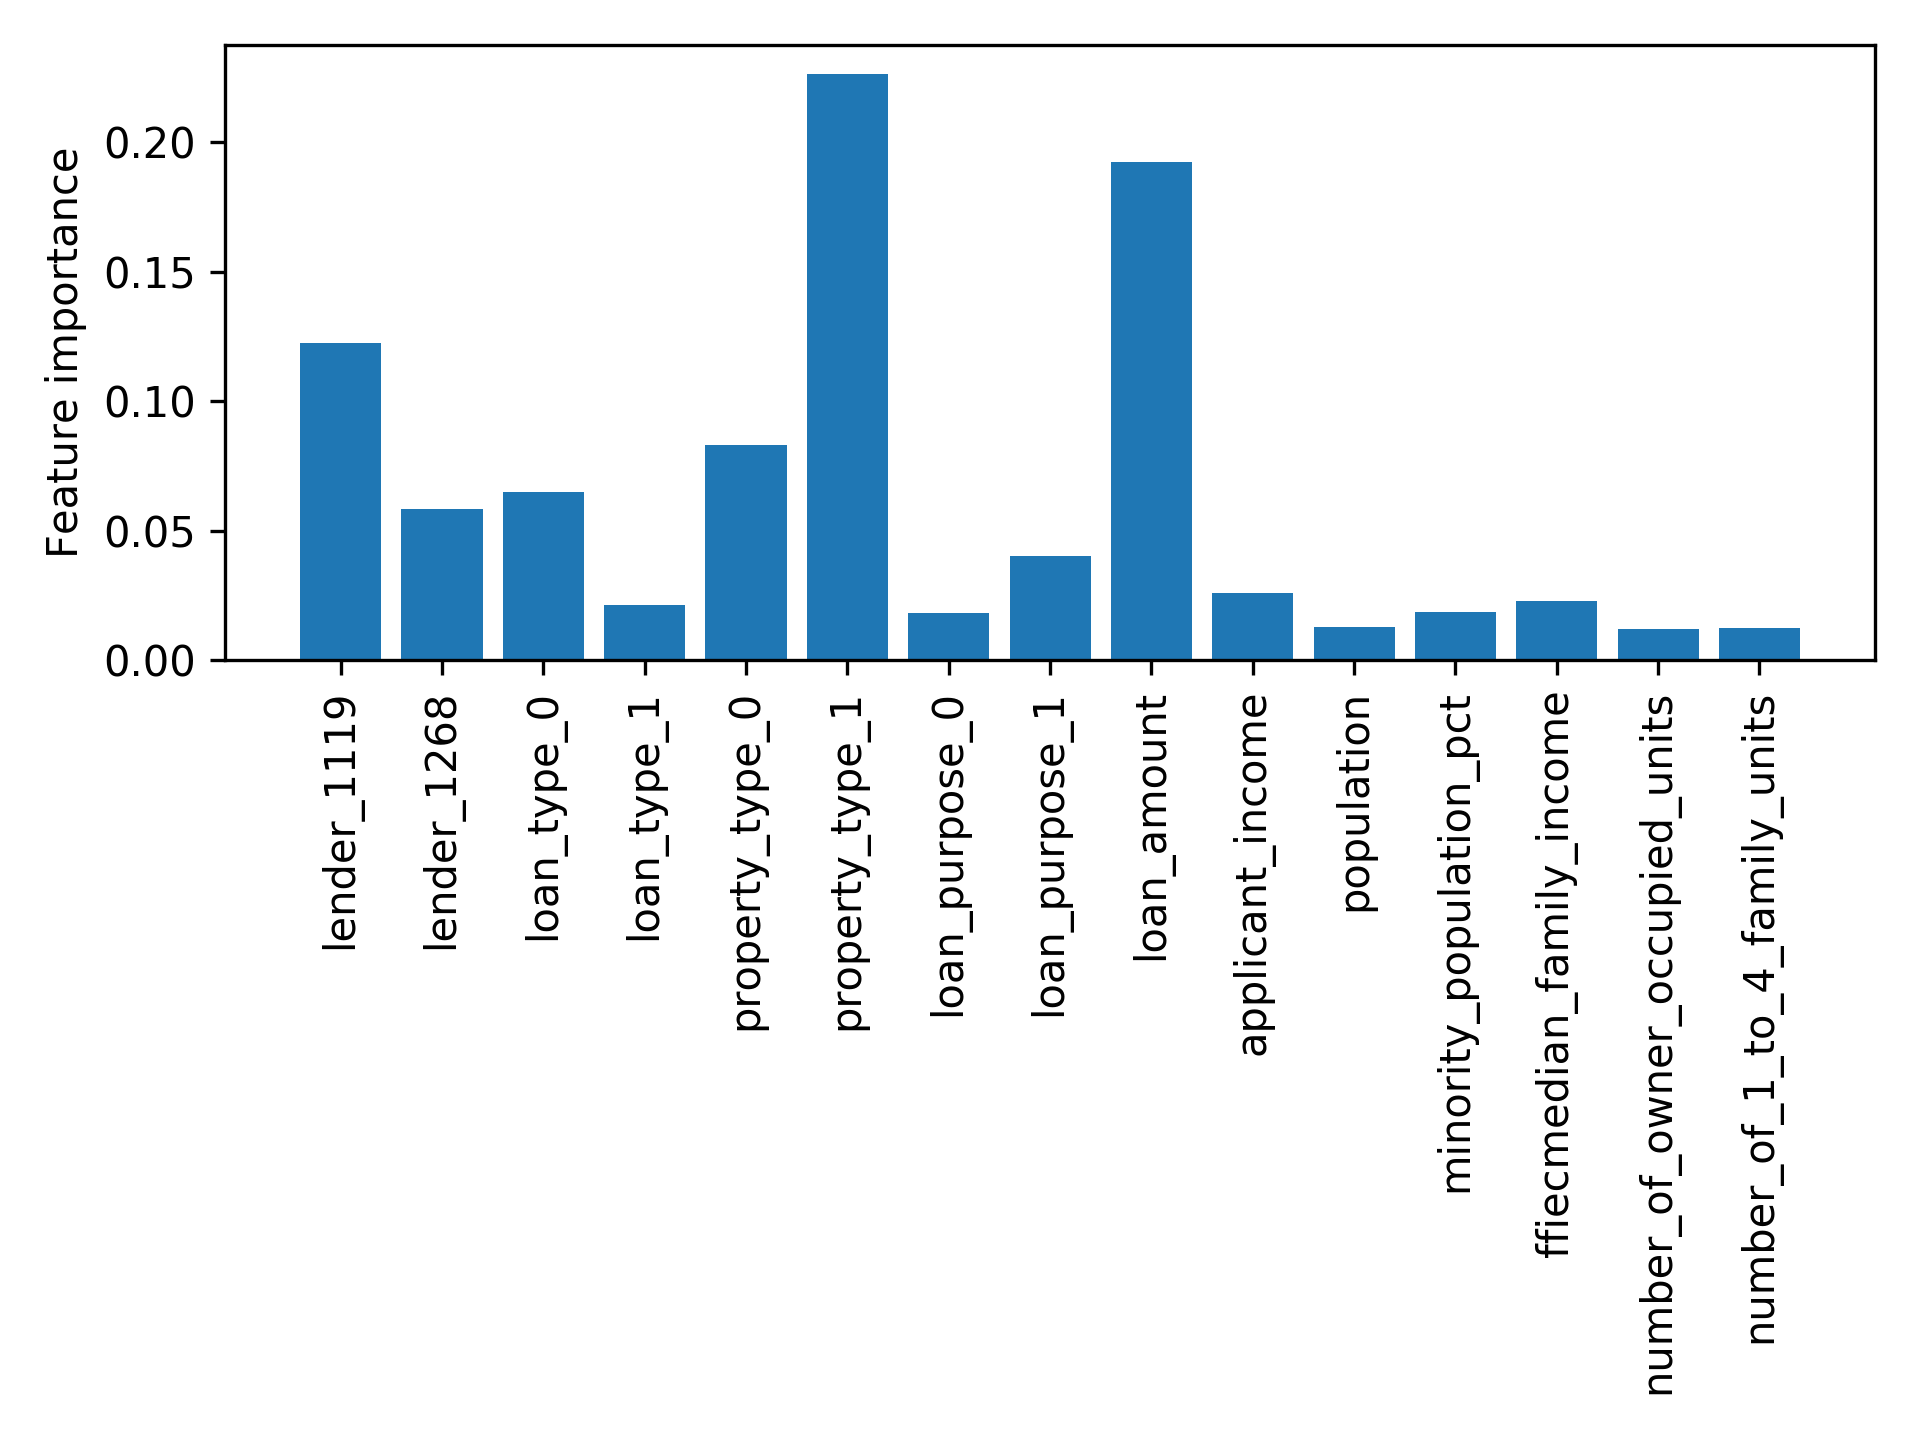
\includegraphics[width=0.6\textwidth]{feature_importance.png}
\caption{Feature importance from random forest regressor modeling. Only features having the highest importance are plotted.}
\label{fig:importance}
\end{figure}



Finally, this trained random forest regressor model was used to predict the rate spread of a new dataset of 200,000 observations. 
Missing values also occur in these new observations. Missing categorical variables were replaced with the most frequent value in training set. Missing numerical values were replaced with the median value in training set. 
What is more, there are some new values in categorical variables (property location: MSA/MD, state and county; lender) that never occur in training set. 
It should be reasonable to treat these values as low frequency values and will be dismissed in prediction. 
The same coding strategy for categorical variables and standardization scales were used to these new observations. 
A prediction to these new observations gave $R^2 = 0.64$.


\section{Conclusions and recommendations}

Based on this analysis and modeling, home mortgage rate can be predicted.
The leading characteristics are property type, lender, loan amount and loan type.
Other features, such as applicant information, demographics and property location are also required for a reliable prediction.
Outlier cases, such as observations with rate spread of 99.0 which is far away from all the other cases, 
need further study to be understood and predicted.


\end{document}
